\begin{figure}[H]
    \caption{A size-8 FFT}
    \begin{center}
        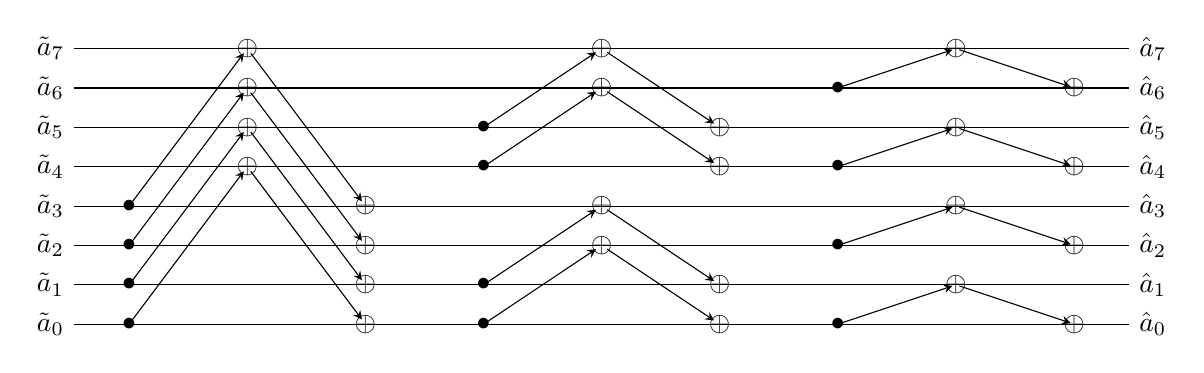
\begin{tikzpicture}[scale=0.5]
            \node (in8) at (0,7) {$\tilde{a}_7$};
            \node (in7) at (0,6) {$\tilde{a}_6$};
            \node (in6) at (0,5) {$\tilde{a}_5$};
            \node (in5) at (0,4) {$\tilde{a}_4$};
            \node (in4) at (0,3) {$\tilde{a}_3$};
            \node (in3) at (0,2) {$\tilde{a}_2$};
            \node (in2) at (0,1) {$\tilde{a}_1$};
            \node (in1) at (0,0) {$\tilde{a}_0$};
            \node (out8) at (28,7) {$\hat{a}_7$};
            \node (out7) at (28,6) {$\hat{a}_6$};
            \node (out6) at (28,5) {$\hat{a}_5$};
            \node (out5) at (28,4) {$\hat{a}_4$};
            \node (out4) at (28,3) {$\hat{a}_3$};
            \node (out3) at (28,2) {$\hat{a}_2$};
            \node (out2) at (28,1) {$\hat{a}_1$};
            \node (out1) at (28,0) {$\hat{a}_0$};


            \node(m1) at (2, 0) {$\bullet$};
            \node(m2) at (11, 0) {$\bullet$};
            \node(m3) at (20, 0) {$\bullet$};
            \node(m4) at (2, 1) {$\bullet$};
            \node(m5) at (11, 1) {$\bullet$};
            \node(m6) at (20, 2) {$\bullet$};
            \node(m7) at (2, 2) {$\bullet$};
            \node(m8) at (11, 4) {$\bullet$};
            \node(m9) at (20, 4) {$\bullet$};
            \node(m10) at (2, 3) {$\bullet$};
            \node(m11) at (11, 5) {$\bullet$};
            \node(m12) at (20, 6) {$\bullet$};

            \node(a1) at (8, 0) {$\oplus$};
            \node(a2) at (17, 0) {$\oplus$};
            \node(a3) at (26, 0) {$\oplus$};
            \node(a4) at (8, 1) {$\oplus$};
            \node(a5) at (17, 1) {$\oplus$};
            \node(a6) at (26, 2) {$\oplus$};
            \node(a7) at (8, 2) {$\oplus$};
            \node(a8) at (17, 4) {$\oplus$};
            \node(a9) at (26, 4) {$\oplus$};
            \node(a10) at (8, 3) {$\oplus$};
            \node(a11) at (17, 5) {$\oplus$};
            \node(a12) at (26, 6) {$\oplus$};

            \node(b1) at (5, 4) {$\oplus$};
            \node(b2) at (14, 2) {$\oplus$};
            \node(b3) at (23, 1) {$\oplus$};
            \node(b4) at (5, 5) {$\oplus$};
            \node(b5) at (14, 3) {$\oplus$};
            \node(b6) at (23, 3) {$\oplus$};
            \node(b7) at (5, 6) {$\oplus$};
            \node(b8) at (14, 6) {$\oplus$};
            \node(b9) at (23, 5) {$\oplus$};
            \node(b10) at (5, 7) {$\oplus$};
            \node(b11) at (14, 7) {$\oplus$};
            \node(b12) at (23, 7) {$\oplus$};

            \draw[-] (in1) -- (out1);
            \draw[-] (in2) -- (out2);
            \draw[-] (in3) -- (out3);
            \draw[-] (in4) -- (out4);
            \draw[-] (in5) -- (out5);
            \draw[-] (in6) -- (out6);
            \draw[-] (in7) -- (out7);
            \draw[-] (in8) -- (out8);

            \draw[-stealth, shorten >=-6.5pt] (m1.center) -- (b1);
            \draw[-stealth, shorten >=-6.5pt, shorten <=-6.5pt] (b1) -- (a1);
            \draw[-stealth, shorten >=-6.5pt] (m2.center) -- (b2);
            \draw[-stealth, shorten >=-6.5pt, shorten <=-6.5pt] (b2) -- (a2);
            \draw[-stealth, shorten >=-6.5pt] (m3.center) -- (b3);
            \draw[-stealth, shorten >=-6.5pt, shorten <=-6.5pt] (b3) -- (a3);
            \draw[-stealth, shorten >=-6.5pt] (m4.center) -- (b4);
            \draw[-stealth, shorten >=-6.5pt, shorten <=-6.5pt] (b4) -- (a4);
            \draw[-stealth, shorten >=-6.5pt] (m5.center) -- (b5);
            \draw[-stealth, shorten >=-6.5pt, shorten <=-6.5pt] (b5) -- (a5);
            \draw[-stealth, shorten >=-6.5pt] (m6.center) -- (b6);
            \draw[-stealth, shorten >=-6.5pt, shorten <=-6.5pt] (b6) -- (a6);
            \draw[-stealth, shorten >=-6.5pt] (m7.center) -- (b7);
            \draw[-stealth, shorten >=-6.5pt, shorten <=-6.5pt] (b7) -- (a7);
            \draw[-stealth, shorten >=-6.5pt] (m8.center) -- (b8);
            \draw[-stealth, shorten >=-6.5pt, shorten <=-6.5pt] (b8) -- (a8);
            \draw[-stealth, shorten >=-6.5pt] (m9.center) -- (b9);
            \draw[-stealth, shorten >=-6.5pt, shorten <=-6.5pt] (b9) -- (a9);
            \draw[-stealth, shorten >=-6.5pt] (m10.center) -- (b10);
            \draw[-stealth, shorten >=-6.5pt, shorten <=-6.5pt] (b10) -- (a10);
            \draw[-stealth, shorten >=-6.5pt] (m11.center) -- (b11);
            \draw[-stealth, shorten >=-6.5pt, shorten <=-6.5pt] (b11) -- (a11);
            \draw[-stealth, shorten >=-6.5pt] (m12.center) -- (b12);
            \draw[-stealth, shorten >=-6.5pt, shorten <=-6.5pt] (b12) -- (a12);
        \end{tikzpicture}
    \end{center}
    \label{fig:fft-full} 
\end{figure}